\documentclass[english]{article}

%%%%%%%%% PACKAGES %%%%%%%%%%%%%%%%%
\usepackage[utf8]{inputenc}
\usepackage[T1]{fontenc}
\usepackage{amsmath}
\usepackage{amssymb}
\usepackage{amsfonts}
\usepackage{alltt}
\renewcommand{\ttdefault}{txtt} % to resolve a problem with bold fonts in alltt

\usepackage{listings}
\lstset{language=haskell,basicstyle=\ttfamily}

\usepackage{proof}
\inferLineSkip=4pt  % increase spacing between lines; default is 2pt

\usepackage[table]{xcolor}
\usepackage[colorlinks,hyperindex,bookmarks,linkcolor=blue,citecolor=blue,urlcolor=blue]{hyperref}
\usepackage{todonotes}

\usepackage{fancyhdr}

%\usepackage{floatflt}
\usepackage{wrapfig}
\usepackage{caption}
\usepackage{subcaption}
\usepackage{framed}
\usepackage{multicol}

\makeatletter

\usepackage{babel}
\usepackage{graphicx}
\usepackage{theorem}

\usepackage{tikz}
\usetikzlibrary{trees}
\usetikzlibrary{positioning} 
\usepackage{tikzsymbols}


\makeatother

%%%%%%%%% GEOMETRY %%%%%%%%%%%%%%%%%
\addtolength{\topmargin}{-15mm}
\addtolength{\textheight}{25mm}
\addtolength{\oddsidemargin}{-20mm}
\setlength{\textwidth}{16cm}

%%%%%%%%% DECLS / DEFNS %%%%%%%%%%%%%%%%%

\usepackage{comment}
\specialcomment{solution}
{\todo[inline]{BEGIN SOLUTION}}
{\todo[inline]{END SOLUTION}}

{\theorembodyfont{\rmfamily} 
  \newtheorem{exo}{Exercise}
  \newtheorem{rem}{Remark}
}

% Macros for references
\newcommand{\polyref}[1]{polycopié, {#1}}

%%%%%%%%% END DECLS / DEFNS %%%%%%%%%%%%%%%%%

%%% Local Variables: 
%%% mode: latex
%%% coding: utf-8-unix
%%% End: 

%======================================================================
%%%%%%%%% DECLS / DEFNS %%%%%%%%%%%%%%%%%

% redefine existing green color
\newcommand{\brightgreen}[1]{{\color{green}#1}}
\definecolor{darkgreen}{rgb}{0,0.7,0}
\newcommand{\green}[1]{{\color{darkgreen}#1}}

\newcommand{\blue}[1]{{\color{blue}#1}}
%\newcommand{\green}[1]{{\color{green}#1}}
\newcommand{\red}[1]{{\color{red}#1}}
\newcommand{\yellow}[1]{{\color{yellow}#1}}
\definecolor{grey}{rgb}{0.5,0.5,0.5}
\newcommand{\grey}[1]{{\color{grey}#1}}
\newcommand{\black}[1]{{\color{black}#1}}

% Logique
\newcommand{\IMPL}[0]{\longrightarrow}
\newcommand{\IMPLL}[0]{\Longrightarrow} % another implication, to make
                                % a difference with reduction relations
\newcommand{\AND}[0]{\land}
\newcommand{\OR}[0]{\lor}
\newcommand{\NOT}[0]{\lnot}
\newcommand{\FALSE}[0]{\perp}
\newcommand{\TRUE}[0]{\top}
\newcommand{\IFF}[0]{\leftrightarrow}
\newcommand{\BIGAND}[1]{\bigwedge_{#1}}
\newcommand{\BIGOR}[1]{\bigvee_{#1}}
\newcommand{\BIGANDC}[2]{\bigwedge_{#1|#2}} % bigand with constraint
\newcommand{\BIGORC}[2]{\bigvee_{#1|#2}}    % bigor with constraint
\newcommand{\ufb}[0]{\mbox{$\stackrel{?}{=}$}} % unifiable

% semantique
\newcommand{\semtrans}[3]{\mbox{$\langle #1, #2 \rangle \rightarrow #3$}}
\newcommand{\statesel}[2]{\mbox{$#1 . #2$}}
\newcommand{\stateupd}[3]{\mbox{$#1 . #2 \leftarrow #3$}}


% Macros for mathematical notation

\def\N{{\mathbf N}}                      % ensemble des entiers naturels
\def\Z{{\mathbf Z}}                      % ensemble des entiers relatifs
\newcommand{\zmod}[1]{\mbox{$ \Z/{#1} \Z$}}  % anneau Z mod m


% WP-calcul
\newcommand{\wpform}[1]{\mbox{\{\( #1 \)\} }}
\newcommand{\subst}[3]{ #1 [ #2 \mbox{$\leftarrow\ $} #3]}
\newcommand{\pfp}[2]{\mbox{\emph{pfp}(\texttt{#1}, \mbox{$#2$})}}
\newcommand{\evb}[1]{\emph{évaluable}($#1$)}

% special references
\newcommand{\secref}[1]{\S~\ref{#1}}
\newcommand{\transpref}[1]{transparent, p.~\ref{#1}}


\newtheorem{theorem}{Théorème}
\newtheorem{lemma}{Lemme}
\newtheorem{definition}{Définition}
\newtheorem{logic}{Principe}


%%% Local Variables: 
%%% mode: latex
%%% TeX-master: "main"
%%% coding: utf-8
%%% End: 


\begin{document}

\begin{center}
  {\LARGE Graph Algorithms in Haskell}
\end{center}


%----------------------------------------------------------------------
\section{Context}\label{sec:context}

The following exercises are thought to elaborate on some of the problems
presented during the talk on graph algorithms. The \LaTeX{} sources of the
slides are available on Github.
\footnote{\url{https://github.com/smucclaw/sandbox/tree/default/martinstrecker/Presentation_2020_12_04_graphs}}
\footnote{Please drop me a line if you have difficulties compiling the \LaTeX{}
  sources, and I will send you the slides.}

After discussing technical issues (\secref{sec:setup}), we will code some
``concrete'' graphs in Haskell and display them with Graphviz
(\secref{sec:graphviz}), and then explore the depth-first-search and
breadth-first-search functions on them (\secref{sec:search_concrete}). Note
that \secref{sec:graphviz} and \secref{sec:search_concrete} are rather
independent from one another, so if you get stuck on the first, continue with
the second.  Finally, we will code the river crossing example
(\secref{sec:river_crossing}) and the $n$-queens example
(\secref{sec:n_queens}).

One reference worth reading is Larry Paulson's \emph{ML for the Working
  Programmer}\footnote{available online:
  \url{https://www.cl.cam.ac.uk/~lp15/MLbook/index.html}}. As the name
suggests, it is written for the ML family of programming languages, which is
altogether not so different from Haskell, with one notable difference: ML
inherently has a \emph{strict} evaluation strategy, which makes dealing with
infinite objects more complex. The discussion of the search algorithms on the
slides owes much to this book (see in particular chapter~5).

%----------------------------------------------------------------------
\section{Setup}\label{sec:setup}

To get everything running, I use the following preamble:

\begin{lstlisting}
{-# OPTIONS_GHC -XFlexibleInstances #-}

module Graphs where

import Data.Maybe
import Data.Text.Lazy as T (pack)

import Data.Graph.Inductive.Graph
import Data.Graph.Inductive.PatriciaTree

import Data.GraphViz
import Data.GraphViz.Printing
import Data.GraphViz.Commands
import Data.GraphViz.Attributes.Complete
\end{lstlisting}

The \texttt{Data.Graph} and \texttt{Data.Graphviz} imports should be clear
from the talk. The remaining imports and the compiler options will be
justified later. Consequently, you will probably also have to add the libraries
\texttt{fgl}, \texttt{graphviz} and \texttt{text} to your dependencies
(\emph{e.g.} \texttt{build-depends} in your \texttt{cabal} file).



%----------------------------------------------------------------------
\section{Graphs in Graphviz}\label{sec:graphviz}

\begin{exo} \
  \begin{enumerate}
  \item The first thing to do is to try to display a small graph in
    Graphviz. For this, code the edge-labelled graph (p. 9 on the slides) as
    described on pp. 14 and 16. When ``running'' the function
    \texttt{smallGrDot}, a file named \texttt{graph.pdf} is generated that can
    be displayed with standard PDF viewers.
  \item For the pleasure of it, you may then code larger graphs (or parts
    thereof),  as the one on p. 5 of the slides. It does not seem to be
    possible to generate non-labelled graphs. In order to omit edge labels,
    you can create a graph of type \texttt{Gr String String} where the label
    component of the edges is the empty string. 
  \end{enumerate}
\end{exo}
As mentioned in the talk, it is inconvenient that one cannot directly refer to
(node) labels when specifying the set of vertices or edges, but one has to
translate these labels to numbers that serve as IDs for the nodes.  Before
starting to code larger graphs for Graphviz, you may prefer to proceed to the
following exercises first.

In the following, we will not use edge-labelled graphs, and instead of
manipulating node IDs, we directly want to manipulate labels. This is more
natural (but slightly less efficient) and without risk as long as node labels
are unique in a graph (there are not two nodes that have the same label). We
also aim at a representation of a graph that is as compact as possible.

To achieve this, we will examine and compare three different representations of graphs:
\begin{enumerate}
\item The \texttt{Gr} graph representation, based on the type \texttt{Gr a b}
  as provided by the \texttt{Data.Graph} and \texttt{Data.GraphViz} libraries,
  presented on the slides and used in the exercise above.
\item An \emph{edge-list} representation, for which we introduce a new type
\begin{lstlisting}
data EdgeListGraph a = ELG [a] [(a, a)]
  deriving (Eq, Ord, Show, Read)
\end{lstlisting}
  
\item A \emph{next-fun} representation which represents edges through a function that
  yields the list of successors of a node. Since it is the most compact
  representation, it is also more fun to work with it! It is defined as:
\begin{lstlisting}
data NextFunGraph a = NFG [a] (a -> [a])
\end{lstlisting}
Because the second argument of the constructor \texttt{NFG} is a function, it
is not possible to inject this type into the \texttt{Eq, Ord, Show, Read} type classes.
\end{enumerate}

Take the following graph from the slides:

\begin{figure}[h]
\begin{center}
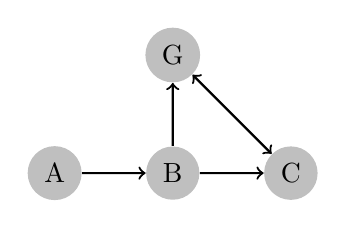
\begin{tikzpicture}[scale=1.5,
on grid,
simple/.style ={shape=circle, fill=grey!50},
blue/.style ={shape=circle, fill=blue!50},
red/.style ={shape=circle, fill=red!50},
auto]

\node[simple] (a) at (0, 1) {A};
\node[simple] (b) at (1, 1) {B};
\node[simple] (c) at (2, 1) {C};
\node[simple] (g) at (1, 2) {G};

\begin{scope}[every path/.style=solid,thick]
\draw[->] (a) -- (b);
\draw[->] (b) -- (c);
\draw[->] (b) -- (g);
\draw[<->] (c) -- (g);
\end{scope}
\end{tikzpicture}
\end{center}
\caption{Small example graph}\label{fig:small_example_graph}
\end{figure}

Its \emph{edge-list} representation is 
\begin{lstlisting}
smallGrELG =
  ELG ["A", "B", "C", "G"] [("A", "B"), ("B", "C"), ("B", "G"), ("C", "G"), ("G", "C")]
\end{lstlisting}

For the \emph{next-fun} representation, we first define the node successor
function:
\begin{lstlisting}
smallGrNexts x = case x of
  "A" -> ["B"]
  "B" -> ["C", "G"]
  "C" -> ["G"]
  "G" -> ["C"]
  _   -> []

smallGrNFG = NFG ["A", "B", "C", "G"] smallGrNexts
\end{lstlisting}


It seems that explicitly representing the node set is superfluous as the
nodes seem to be inferrable from the edges. But this is not so. Why? Note that
our graphs can be broken into separate disconnected islands; in particular,
there may be isolated nodes without incoming or outgoing edges.

We now provide conversions between these types.


\begin{exo}\label{exo:edgeListGraphToGr}
Write a function \texttt{edgeListGraphToGr} that translates an edge-list graph
to a \texttt{Gr} graph representation. Its type is:

\begin{lstlisting}
edgeListGraphToGr :: (Eq a) => EdgeListGraph a -> Gr a String
\end{lstlisting}
Indeed, the node label type \texttt{a} has to be an equality type because
otherwise, we cannot know whether to node labels are mapped to the same node
ID.

Some hints:
\begin{itemize}
\item Write an auxiliary function that maps the nodes:
\begin{lstlisting}
  edgeListGraphToGrNodes :: [a] -> [LNode a]
\end{lstlisting}
so that \texttt{edgeListGraphToGrNodes ["A", "B", "C", "G"]} is
\texttt{[(0,"A"),(1,"B"),(2,"C"),(3,"G")]}.
Remember that \texttt{LNode a} is just the pair  \texttt{(Node, a)}, where
\texttt{Node} is a synonym for \texttt{Int}. 
Think of using the \texttt{zip} function. And there is an easy way of writing
a list of consecutive numbers: for example, \texttt{[0,1,2,3]} is written
\texttt{[0 .. 3]}.

\item Write an auxiliary function that maps the edges, from \texttt{[(a, a)]}
  to \texttt{[LEdge String]}. 
  For example, it will have to translate the edge \texttt{("B", "C")} to
  \texttt{(1, 2, "")}. To do so, it is useful to take the swapped list of
  \texttt{edgeListGraphToGrNodes}, namely
  \texttt{[("A",0),("B",1),("C",2),("G",3)]}, and ``apply'' it to the edge list.
\end{itemize}
\end{exo}


\begin{exo}\label{exo:nextFunGraphToEdgeListGraph}
Now, let's 
write a function \texttt{nextFunGraphToEdgeListGraph} that translates a
next-fun graph to an edge-list graph:
\begin{lstlisting}
nextFunGraphToEdgeListGraph :: NextFunGraph a -> EdgeListGraph a
\end{lstlisting}

Hint: write an auxiliary function
\begin{lstlisting}
edgeNextsToEdgeList :: (a -> [a]) -> [a] -> [(a, a)]
\end{lstlisting}
that takes a \emph{nexts} function (such as \texttt{smallGrNexts}) and a list
of nodes (such as \texttt{["A", "B", "C", "G"]}) and produces the
corresponding edge list: \texttt{edgeNextsToEdgeList smallGrNexts ["A", "B", "C", "G"]} yields 
\texttt{[("A","B"),("B","C"),("B","G"),("C","G"),("G","C")]}.
\end{exo}

Instead of the unintuitive definition of \texttt{smallGraph} as on the slides
p. 14, we can now use the chain of conversions and define:
\begin{lstlisting}
smallGraph :: Gr String String
smallGraph =
  edgeListGraphToGr (nextFunGraphToEdgeListGraph
                     (NFG ["A", "B", "C", "G"]  smallGrNexts))

smallGrDot :: IO FilePath
smallGrDot = runGraphviz (graphToDot quickParams smallGraph) Pdf "graph.pdf"         
\end{lstlisting}
and finally run \texttt{smallGrDot} for the display.

You are now well prepared to code the more complex graphs that appear on the
slides, and to visualize them in Graphviz.

%----------------------------------------------------------------------
\section{Search in Concrete Graphs}\label{sec:search_concrete}

You can start working on this section without having completed
\secref{sec:graphviz}, but you maybe have to refer to some definitions of
\secref{sec:graphviz}.

The \emph{next-fun} representation of edges has the advantage that we can use
the function directly in the search procedures, such as the following, where
we look for paths from \texttt{A} to \texttt{G}:

\begin{lstlisting}
> take 5 (breadthfirst smallGrNexts (== "G") "A")
["G","G","G","G","G"]
\end{lstlisting}
Remember that \texttt{take $n$} fetches the $n$ first elements of a (possibly
infinite) list.  The result is interesting in that it shows that there are at least 5
paths from \texttt{A} to \texttt{G}, but is otherwise a bit disappointing
because it does not show us the paths.

Let us define a search path as a list of nodes:
\begin{lstlisting}
type SearchPath a = [a]
\end{lstlisting}
By convention, the start node of the path will be the first of the list and
the node reached by the path the last one.

In order to use the search procedures, we will now ``lift'' the \emph{nexts}
function on paths, in the following sense: suppose we are given a path, such as
\texttt{["A", "B"]}, which says that we have travelled from \texttt{A} to
\texttt{B}. The lift will give us the list of paths we obtain when going one
step further, for example:

\begin{lstlisting}
> liftNextsToPath smallGrNexts ["A", "B"]
[["A","B","C"],["A","B","G"]]
\end{lstlisting}


\begin{exo}\label{exo:liftNextsToPath}
Write function
\begin{lstlisting}
liftNextsToPath :: (a -> [a]) -> SearchPath a -> [SearchPath a]
\end{lstlisting}
\end{exo}

We can now define 

\begin{lstlisting}
pathsFromToBFS nexts start goal =
  breadthfirst
  (liftNextsToPath nexts)
  (\pth -> last pth == goal)
  [start]
\end{lstlisting}
(and similarly for depth-first search) that has a more satisfactory behaviour:

\begin{lstlisting}
> take 5 (pathsFromToBFS smallGrNexts "A" "G")
[["A","B","G"],
 ["A","B","C","G"],
 ["A","B","G","C","G"],
 ["A","B","C","G","C","G"],
 ["A","B","G","C","G","C","G"]]
\end{lstlisting}

There is however still something wrong with this definition. If you run the
search in the opposite direction: \texttt{(pathsFromToBFS smallGrNexts "G" "A")},  
it will not terminate. Before reading on, please try to understand
what is going on and which feature causes non-termination.

If there are no paths between two nodes, we would like the procedure to
terminate with an empty list and not to continue searching endlessly. 
The solution we propose comes at the price of not admitting cycles in the
paths we generate. A \emph{cycle} is a path which visits at least one node
several times, and for many applications, cycles are indeed useless.


\begin{exo}\label{exo:liftNextsToPathNoDup}
Write function
\begin{lstlisting}
liftNextsToPathNoDup :: (a -> [a]) -> SearchPath a -> [SearchPath a]
\end{lstlisting}
that lifts a \emph{nexts} function to a search path without duplicates, thus omitting cyclic paths.
\end{exo}

It has the following behaviour:
\begin{lstlisting}
> liftNextsToPathNoDup smallGrNexts ["A","B","G"]
[["A","B","G","C"]]
> liftNextsToPathNoDup smallGrNexts ["A","B","G","C"]
[]
\end{lstlisting}
In the first case, the function behaves as \texttt{liftNextsToPath}, but in
the second case, it refuses to construct the path
\texttt{["A","B","G","C","G]} which would be cyclic.

Now, replace  \texttt{liftNextsToPath} by  \texttt{liftNextsToPathNoDup} in
the definition of \texttt{pathsFromToBFS} and its depth-first-search
counterpart \texttt{pathsFromToDFS}, and \texttt{(pathsFromToBFS smallGrNexts
  "G" "A")} will terminate with an empty list.

%----------------------------------------------------------------------
\section{River Crossing}\label{sec:river_crossing}

The scenario of this puzzle is the following: a cabbage, a ferryman, a goat
and a wolf are on the left side of a river and want to cross it, \emph{i.e.}
all the four should eventually be on the right side of the river. There is a
boat that can carry at most two of the four parties, and only the ferryman can
row it. Of course, the boat cannot cross without a passenger, but the ferryman
can travel alone. For obvious reasons, the cabbage and the goat cannot be left
alone without the surveillance of the ferryman, and neither can the wolf and
the goat.

In order to model the situation, we introduce the following definitions:
\begin{lstlisting}
data Side = Ls | Rs
  deriving (Eq, Ord, Show, Read)

type CfgwState = (Side, Side, Side, Side)
\end{lstlisting}

The state codes the sides where the cabbage, ferryman, goat and wolf (in this
order) are positioned. Thus, in \texttt{(Ls, Rs, Ls, Rs)}, the cabbage and
goat are on the left and the ferryman and the wolf on the right (and this
would not be a valid state according to the above constraints).

\begin{exo}\label{exo:cross}
  Write functions \texttt{crossCabbage, crossFerryman, crossGoat, crossWolf},
  all of type \texttt{CfgwState -> CfgwState}, that describe the crossing of
  each of these personalities. Thus, \texttt{crossCabbage (Ls, Rs, Ls, Rs)}
  gives \texttt{(Rs, Rs, Ls, Rs)} (never mind that the cabbage cannot cross
  alone, see exercise~\ref{exo:crossBoat}).
\end{exo}

\begin{exo}\label{exo:validState}
  Write function \texttt{validState :: CfgwState -> Bool} that verifies that a
  state satisfies the constraints of simultaneous presence of cabbage and goat
  resp. goat and wolf on one side.
\end{exo}

\begin{exo}\label{exo:crossBoat}
  Write function \texttt{crossBoat :: CfgwState -> [CfgwState]} that, given a
  state, produces all follow-up states provided:
  \begin{itemize}
  \item the crossings correspond to valid boat movements (either the ferryman
    alone, or the ferryman with one of the other three beings);
  \item the states attained are valid in the sense of exercise~\ref{exo:validState}.
  \end{itemize}
  For example, \texttt{crossBoat (Ls, Ls, Ls, Rs)} gives
  \texttt{[(Rs,Rs,Ls,Rs),(Ls,Rs,Rs,Rs)]}. The state \texttt{(Rs, Ls, Ls, Rs)}
  cannot be reached because the cabbage cannot travel alone. The state
  \texttt{(Ls, Rs, Ls, Rs)} cannot be reached because cabbage and goat would
  be alone on the left side.

  \emph{Hints:}
  \begin{itemize}
  \item See how you can describe the simultaneous movement of two actors by
    function composition (the ``dot'' function \texttt{.}) of the crossing
    functions of exercise~\ref{exo:cross}.
  \item If you have ever wondered what the \texttt{Applicative} type class is
    good for: here is a good place to use it, in particular the operator
    \texttt{(<*>) :: Applicative f => f (a -> b) -> f a -> f b}. Try out what
    happens if you have a
    list of functions and a list of elements, such as: \texttt{[(+ 1), (* 2),
      (+ 7)] <*> [42]}. Establish the correspondence with the different crossing functions.
  \item To filter out the valid states, not surprisingly, use the \texttt{filter} function.
  \end{itemize}
\end{exo}

\begin{exo}\label{exo:cfgwSearch}
  It is now easy to use the functions \texttt{pathsFromToBFS} or
  \texttt{pathsFromToDFS} to obtain the sequence of states that solves the
  puzzle (there are two possible paths). Of course, \texttt{crossBoat} is the
  \emph{nexts}-function; now you only have to specify the start and goal state.
\end{exo}

To display the search graph, we would like to proceed as before: First define
a graph in \emph{next-fun} representation, convert it to \emph{edge-list} and
then \texttt{Gr} graph representation and finally display it (compare the
definition of \texttt{smallGrDot} in \secref{sec:graphviz}). For this, we
first need the node set of the search graph.

\begin{exo}\label{exo:cfgwDot}
  Define \texttt{cfgwNodes :: [CfgwState]} as the list of possible states. You
  have the following alternatives:
  \begin{enumerate}
  \item As components of the quadruple, take all possible combinations of
    \texttt{Ls} and \texttt{Rs}, which will produce $2^4=16$ states, among
    them also states that are not valid. This will give you the graph
    displayed on the slides.
  \item Restrict yourself to the combinations that form a valid state, of
    which there are 10.
  \end{enumerate}
\end{exo}

We would now like to make the following definitions:

\begin{lstlisting}
cfgwGraph = edgeListGraphToGr (nextFunGraphToEdgeListGraph (NFG cfgwNodes crossBoat))
cfgwDot = runGraphviz (graphToDot quickParams cfgwGraph) Pdf "graph.pdf"
\end{lstlisting}

It turns out that Haskell complains (``No instance for (Labellable CfgwState)
arising from a use of ‘quickParams’ '') because it does not know how to render
a \texttt{CfgwState} in Graphviz. To make a long story short: add the
following declaration to get rid of the error:\footnote{It is due to this
  declaration that the compiler option and the remaining imports are required
  in the preamble of the module.}
\begin{lstlisting}
instance Labellable CfgwState where
  toLabelValue s  = StrLabel (T.pack (show s))
\end{lstlisting}
Now, the above definitions are possible, and you can display the graph.

%----------------------------------------------------------------------
\section{$n$-Queens}\label{sec:n_queens}

\begin{figure}[t]
\begin{center}
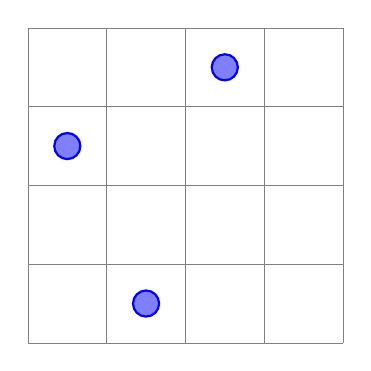
\begin{tikzpicture}[
simple/.style ={shape=circle, fill=grey!50},
blue/.style ={shape=circle, thick, draw=blue!100, fill=blue!50},
auto]
\draw[help lines] (0,0) grid (4,4);
%\fill (1cm,1.5cm) blue (5pt);
\node[blue] (a) at (0.5, 2.5) { };
\node[blue] (b) at (1.5, 0.5) { };
\node[blue] (c) at (2.5, 3.5) { };
\end{tikzpicture}
\end{center}
\caption{Partial solution for the $4$-queens problem}\label{fig:fourqueens}
\end{figure}


The following is a rough sketch how to solve the $n$-queens problem, of which
you also find a good description in Paulson's \emph{ML for the Working
  Programmer} cited in the introduction. The problem is to position $n$ queens on
an $n \times n$ chequerboard so that no queen may attack one another, and this
happens if two queens are on the same row, column or diagonal. 

For finding  solutions, we again use breadth (or depth) first search. There is
a uniquely defined start state of the search (the empty chequerboard), but
contrary to the graph search we have considered, the goal is not a single
state, but rather characterised by a predicate (the \texttt{sol} parameter of
the search procedures).

The idea is to progressively fill the columns with queens until all columns
are filled. Figure~\ref{fig:fourqueens} shows a partial solution, where 3 of
the 4 queens have been placed. As no two queens can occur in one column, it
will be sufficient to record in which row a queen is placed. The situation of
Figure~\ref{fig:fourqueens} can thus be represented by the list \texttt{[2, 4,
  1]}, and the list \texttt{[2, 4, 1, 3]} would be a solution of the problem. 

We let you figure out the details, but keep in mind that the problem has a
high combinatorial complexity: in a brute-force approach, for an $n$-queens
problem, you will generate $n^n$ nodes. When specifying the
\emph{nexts}-function, it is therefore essential to correctly \emph{prune} the
search space: do not fill up the chequerboard with queens and eliminate unsafe
configurations at the end, but already remove a partial solution as soon as is
turns out to be infeasible.

You can comfortably compute all 92 solutions for the 8-queens problem or all
14200 solutions for the 12-queens problem. This should not take more than a
few seconds. Things become worse very quickly for larger numbers of $n$, see
the statistics.\footnote{\url{http://www.durangobill.com/N_Queens.html} - thanks to Jacob Tan for the reference.}

\end{document}






%%% Local Variables: 
%%% mode: latex
%%% TeX-master: t
%%% coding: utf-8-unix
%%% End: 
